\documentclass{article}
\usepackage{tikz}
\usetikzlibrary{patterns, decorations.pathmorphing, arrows.meta}
\newcommand{\pyvar}[1]{\texttt{#1}}
\usepackage{graphicx,scalerel}
\usepackage{adjustbox}
\usetikzlibrary{calc}
\begin{document}



\begin{figure}[h]
    \centering
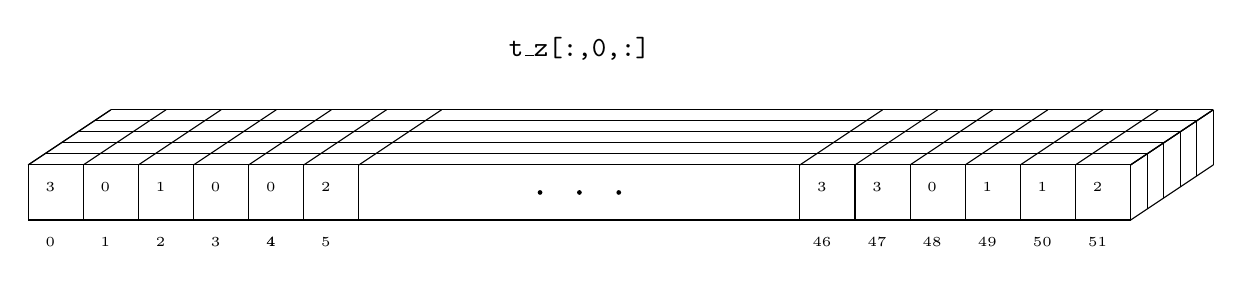
\begin{tikzpicture}
    % Define grid dimensions
    \def\n{1} % N = 1 row (front face height)
    \def\m{20} % M = 20 columns (front face width)
    \def\depth{5} % Depth of the cube (z-axis, number of cells in depth)
    \def\cellsize{0.7} % Size of each cell

    % Define 3D perspective skew for top and right faces
    \def\skewx{0.3} % Skew factor for x-axis (right face)
    \def\skewy{0.2} % Skew factor for y-axis (top face)

    % --- Front Face (the original 1x20 grid) ---
    % Draw the grid - Horizontal lines
    \foreach \i in {0,...,\n} {
        \draw[black] (0,\i*\cellsize) -- (\m*\cellsize,\i*\cellsize); % Horizontal lines
    }

    % Draw the grid - Vertical lines with condition
    \foreach \j in {0,...,\m} {
        \ifnum\j<7 % Check if j < 7
            \draw[black] (\j*\cellsize,0) -- (\j*\cellsize,\n*\cellsize); % Draw line
        \else
            \ifnum\j>13 % Check if j > 13
                \draw[black] (\j*\cellsize,0) -- (\j*\cellsize,\n*\cellsize); % Draw line
            \fi
        \fi
    }

    % Place dots in the middle of the front face (simulating row 3 in a 5-row grid, but here it's the only row)
    \foreach \j in {0,1,2} {
        \fill[black] ({(1-\j)/2+\m*\cellsize/2}, 0.5*\cellsize) circle (0.03); % Dots
    }

    % Draw the outer rectangle for the front face
    \draw[black] (0,0) rectangle (\m*\cellsize, \n*\cellsize);

    % Add the shape label below the grid
    \node[below] at ({\m/2*\cellsize}, 3.5*\cellsize) {\pyvar{t\_z[:,0,:]}};


    \node at (0.4*\cellsize, \n*\cellsize-0.4*\cellsize) {\tiny 3};
    \node at (1.4*\cellsize, \n*\cellsize-0.4*\cellsize) {\tiny 0};
    \node at (2.4*\cellsize, \n*\cellsize-0.4*\cellsize) {\tiny 1};
    \node at (3.4*\cellsize, \n*\cellsize-0.4*\cellsize) {\tiny 0};
    \node at (4.4*\cellsize, \n*\cellsize-0.4*\cellsize) {\tiny 0};
    \node at (5.4*\cellsize, \n*\cellsize-0.4*\cellsize) {\tiny 2};

    \node at (14.4*\cellsize, \n*\cellsize-0.4*\cellsize) {\tiny 3};
    \node at (15.4*\cellsize, \n*\cellsize-0.4*\cellsize) {\tiny 3};
    \node at (16.4*\cellsize, \n*\cellsize-0.4*\cellsize) {\tiny 0};
    \node at (17.4*\cellsize, \n*\cellsize-0.4*\cellsize) {\tiny 1};
    \node at (18.4*\cellsize, \n*\cellsize-0.4*\cellsize) {\tiny 1};
    \node at (19.4*\cellsize, \n*\cellsize-0.4*\cellsize) {\tiny 2};

    % --- Top Face ---
    % Draw the top face as a parallelogram
    \draw[black] (\m*\cellsize, \n*\cellsize) -- ++(\depth*\cellsize*\skewx, \depth*\cellsize*\skewy); % Right edge of top face
    \draw[black] (0, \n*\cellsize) -- ++(\depth*\cellsize*\skewx, \depth*\cellsize*\skewy); % Left edge of top face
    \draw[black] (\m*\cellsize, \n*\cellsize) -- (0, \n*\cellsize); % Front edge (already drawn)
    \draw[black] (\m*\cellsize+\depth*\cellsize*\skewx, \n*\cellsize+\depth*\cellsize*\skewy) -- (0+\depth*\cellsize*\skewx, \n*\cellsize+\depth*\cellsize*\skewy); % Back edge

    % Draw grid lines on the top face (along x-axis)
    \foreach \j in {0,...,\m} {
        \ifnum\j<7 % Same condition as front face
            \draw[black] (\j*\cellsize, \n*\cellsize) -- ++(\depth*\cellsize*\skewx, \depth*\cellsize*\skewy);
        \else
            \ifnum\j>13
                \draw[black] (\j*\cellsize, \n*\cellsize) -- ++(\depth*\cellsize*\skewx, \depth*\cellsize*\skewy);
            \fi
        \fi
    }

    % Draw grid lines on the top face (along z-axis, depth)
    \foreach \k in {0,...,\depth} {
        \draw[black] (\m*\cellsize+\k*\cellsize*\skewx, \n*\cellsize+\k*\cellsize*\skewy) -- (0+\k*\cellsize*\skewx, \n*\cellsize+\k*\cellsize*\skewy);
    }

    % --- Right Face ---
    % Draw the right face as a parallelogram
    % \draw[lightgray] (\m*\cellsize, \n*\cellsize) -- ++(\depth*\cellsize*\skewx, -\depth*\cellsize*\skewy); % Top edge of right face
    % \draw[lightgray] (\m*\cellsize, 0) -- ++(\depth*\cellsize*\skewx, -\depth*\cellsize*\skewy); % Bottom edge of right face
    \draw[black] (\m*\cellsize, \n*\cellsize) -- (\m*\cellsize, 0); % Front edge (already drawn)
    % \draw[lightgray] (\m*\cellsize+\depth*\cellsize*\skewx, \n*\cellsize-\depth*\cellsize*\skewy) -- (\m*\cellsize+\depth*\cellsize*\skewx, -\depth*\cellsize*\skewy); % Back edge

    % Draw grid lines on the right face (along y-axis, height)
    \foreach \i in {0,...,\n} {
        \draw[black] (\m*\cellsize, \i*\cellsize) -- ++(\depth*\cellsize*\skewx, \depth*\cellsize*\skewy);
    }

\foreach \k in {0,...,\depth} {
    \draw[black] (\m*\cellsize+\k*\cellsize*\skewx, \n*\cellsize+\k*\cellsize*\skewy) -- (\m*\cellsize+\k*\cellsize*\skewx, 0+\k*\cellsize*\skewy);
}

    \node at (0.4*\cellsize, \n*\cellsize-1.4*\cellsize) {\tiny 0};
    \node at (1.4*\cellsize, \n*\cellsize-1.4*\cellsize) {\tiny 1};
    \node at (2.4*\cellsize, \n*\cellsize-1.4*\cellsize) {\tiny 2};
    \node at (3.4*\cellsize, \n*\cellsize-1.4*\cellsize) {\tiny 3};
    \node at (4.4*\cellsize, \n*\cellsize-1.4*\cellsize) {\tiny 4};
    \node at (4.4*\cellsize, \n*\cellsize-1.4*\cellsize) {\tiny 4};
    \node at (5  .4*\cellsize, \n*\cellsize-1.4*\cellsize) {\tiny 5};

    \node at (14.4*\cellsize, \n*\cellsize-1.4*\cellsize) {\tiny 46};
    \node at (15.4*\cellsize, \n*\cellsize-1.4*\cellsize) {\tiny 47};
    \node at (16.4*\cellsize, \n*\cellsize-1.4*\cellsize) {\tiny 48};
    \node at (17.4*\cellsize, \n*\cellsize-1.4*\cellsize) {\tiny 49};
    \node at (18.4*\cellsize, \n*\cellsize-1.4*\cellsize) {\tiny 50};
    \node at (19.4*\cellsize, \n*\cellsize-1.4*\cellsize) {\tiny 51};
    
\end{tikzpicture}
\caption{\small Tensor \pyvar{t\_z[:,0,:]} represents the cards laid in the pool and held by Alex and Bob. For example, \pyvar{t\_z[0,0,0]=3}, \pyvar{t\_z[0,0,2]=1}, and \pyvar{t\_z[0,0,51]=2} indicate that the pool contains $A\clubsuit$, Alex holds $A\heartsuit$, and Bob holds $K\spadesuit$, respectively.}
    \label{fig:card_cube}
\end{figure}



\end{document}
